\documentclass{beamer}

\mode<presentation>
{
  \setbeamertemplate{background canvas}[vertical shading][bottom=red!10,top=blue!10]
  \setbeamertemplate{blocks}[rounded][shadow=true]
  \usetheme{Warsaw}
  \setbeamercovered{transparent}
  \usefonttheme[onlysmall]{structurebold}
}


\usepackage[english]{babel}
\usepackage[latin1]{inputenc}
\usepackage{times}
\usepackage[T1]{fontenc}
\usepackage{listings}
\lstloadlanguages{Perl,bash}
\lstset{language=Perl,numbers=left, numberstyle=\tiny, stepnumber=1, numbersep=5pt,
        frame=lines, captionpos=b, basicstyle=\scriptsize}


\title{A Quick Guide to Perl}
\author{Yubao Liu \\ \texttt{liuyb@yahoo-inc.com}}
\institute{Yahoo! Global R \& D Center, Beijing}
\date{2010-09-13}


\hypersetup{pdfpagemode=FullScreen}
\subject{A Quick Guide to Perl}

%\pgfdeclareimage[height=0.5cm]{yahoo-logo}{yahoo-logo.jpg}
%\logo{\pgfuseimage{yahoo-logo}}

\AtBeginSubsection[]
{
  \begin{frame}<beamer>{Outline}
    \tableofcontents[currentsection,currentsubsection]
  \end{frame}
}


\begin{document}

\begin{frame}
  \titlepage
\end{frame}

\begin{frame}{Outline}
  \tableofcontents
  % You might wish to add the option [pausesections]
\end{frame}


\section{Basic Perl}
\subsection{Documentation}

\begin{frame}{Perl - Practical Extraction and Report Language}
  \begin{itemize}
    \item Created by Larry Wall at 1987
    \item Combines some of best features of C, sed, awk and sh
    \item The camel book ``Programming Perl''
    \item 18325 modules on \url{http://www.cpan.org/}
    \item Perl 5.12.2 released at 7th Sep, 2010
    \item Rakudo Star released at 29th Jul, 2010
  \end{itemize}
\end{frame}

\begin{frame}{Successful Stories}
    \begin{center}
    Bugzilla, Request Tracker,
    TWiki (Foswiki),
    MovableType,
    Webmin,
    SVK,
    ack-grep,
    \url{http://slashdot.org/},
    Majordomo, SpamAssassin,
    AWStats, MRTG,
    Perlbal, Mogilefs,
    BioPerl
  \end{center}
\end{frame}

\begin{frame}[containsverbatim]{Hello World!}
\begin{lstlisting}[caption=Greeting from Perl]
#!/usr/bin/perl
use strict;
use warnings;

greet();
exit(0);

sub greet {
    print "Hello world!\n";
}
\end{lstlisting}

Running: \texttt{perl hello.pl}
\end{frame}


\begin{frame}{Recommended Readings}
  \begin{itemize}
    \item Learning Perl, 5th Edition
    \item Advanced Perl Programming, 1st Edition
    \item \url{http://www.pgsqldb.org/mwiki/index.php/ProgrammingPerl}
    \item \url{http://wiki.perlchina.org}
    \item \texttt{perldoc perl}
  \end{itemize}
\end{frame}

\begin{frame}{Access Perl Documents Easily}
  \begin{itemize}
    \item   \url{http://www.perl.org/docs.html}
    \item   \url{http://search.cpan.org/}
    \item   PodBrowser
    \item   Pod::POM::Web
    \item   Pod::Browser
  \end{itemize}
\end{frame}

\subsection{Syntax}

\begin{frame}{Data Types}
  \begin{description}
    \item[Scalar]   \texttt{\$var}, number, string, reference
    \item[Array]    \texttt{@var}, any type
    \item[Hash]     \texttt{\%var}, map from number or string to scalar
    \item[File handle] \texttt{FH}, created by open() and sysopen()
    \item[Typeglob]    \texttt{*symbol}, used to manipulate symbol table
  \end{description}
\end{frame}


\begin{frame}{Scalar}
  \begin{itemize}
    \item Automatically conversion between number and string
    \item \texttt{10/3} gets a float point number, use int() for integer
    \item Interpolation
    \item + . x ++, different logic operators for numbers and strings
    \item \$\_
    \item undef(), defined(), \texttt{perldoc perlsyn}, /Truth and Falsehood
    \item substr(), vec()
    \item octets and strings, length(), use Encode, use encoding, use utf8
  \end{itemize}
\end{frame}


\begin{frame}{Array}
  \begin{itemize}
    \item @a, \$a[0], \$\#a, scalar(@a), (elemA, elemB)
    \item @\_, modify parameters
    \item push(), pop(), shift(), unshift(), splice(),
    \item (\$i, \$j) = (\$j, \$i); (\$a, @a, \$b) = @b
    \item Interpolation: \texttt{"@a"}
    \item Sequence generator: 1..100
    \item Array slice: @a[@b]
  \end{itemize}
\end{frame}

\begin{frame}{Hash}
  \begin{itemize}
    \item \%a, \$\{"key"\}, ("key", "val"), (key => "val")
    \item keys(), values(), each(), exists(), delete()
    \item Hash slice: @h\{@k\}
    \item Key \emph{must} be number or string, value \emph{must} be scalar
  \end{itemize}
\end{frame}

\begin{frame}{typeglob}
  \begin{itemize}
    \item \texttt{perldoc perldata}, \texttt{perldoc perlmod}
    \item To transfer file handles, manipulate symbol table
  \end{itemize}
\end{frame}

\begin{frame}{File handle}
  \begin{itemize}
    \item \texttt{perldoc -f open}, \texttt{perldoc perlopentut}
    \item File handle, reference to file handle, IO::Handle object
  \end{itemize}
\end{frame}

\begin{frame}{Variable declaration}
  \begin{description}
    \item[my]       Lexically scoped local variable
    \item[state]    Lexically scoped static local variable
    \item[local]    Dynamically scoped local variable
    \item[our]      Lexically scoped package variable
    \item[use vars] Package scoped package variable
  \end{description}
\end{frame}

\begin{frame}{Contexts}
  \begin{itemize}
    \item Void context, \texttt{print "...."}
    \item Scalar context, \texttt{\$i < @a; \$i < scalar(@a);}
    \item Array context, \texttt{(stat \$f)[7]}
    \item Numeric context, \texttt{\$a + \$b}
    \item String context, \texttt{\$a\ .\ \$b}
    \item Dual var, \texttt{\$!, Scalar::Util::dualvar()}
    \item wantarray()
  \end{itemize}
\end{frame}

\begin{frame}{Statement}
  \begin{itemize}
    \item \texttt{perldoc perlsyn}
    \item if elsif else, unless, given when
    \item while, until, for, foreach
    \item next, last, redo
    \item do while, do until (\emph{double scopes for next/last/redo!})
    \item goto-LABEL, goto-EXPR, goto-\&NAME
    \item Statement modifiers: \texttt{print \$i++ while \$i < 10;}
    \item BEGIN {...}, END {...}
  \end{itemize}
\end{frame}

\begin{frame}{Comment}
  \begin{itemize}
    \item Single line comment: \#
    \item Trick for multi line comment: =pod .... =cut
  \end{itemize}
\end{frame}

\begin{frame}{Operators and Special Variables}
  \begin{itemize}
    \item \texttt{perldoc perlop}
    \item \texttt{perldoc perlvar}
  \end{itemize}
\end{frame}

\begin{frame}{Subroutine}
  \begin{itemize}
    \item \texttt{perldoc perlsub}
    \item \texttt{perldoc perlfunc}
    \item Omission of \& and parentheses
  \end{itemize}
\end{frame}

\begin{frame}{Reference}
  \begin{itemize}
    \item \texttt{perldoc perlref,perlreftut,perldsc,perllol}
    \item Reference: $\backslash$\$a, $\backslash$@a, $\backslash$\%h, $\backslash$\&name, sub \{...\}
    \item Dereference: \$\$a, @\$a, \$a->[0], \%\$h, \$h->\{"key"\}, \\
          \&\$name(), \$name->()
    \item \$\{\$a[0]\}, \@\{\$a[0]\}, \%\{\$a[0]\}
    \item {}[1, 2, 3], \{a => 1, b => 2\}
    \item Autovivification: \texttt{my \$a; \$a->[0][0][1] = 3;}, \\
          \texttt{$\backslash$( @h\{@k\} )}
  \end{itemize}
\end{frame}

\begin{frame}{I/O}
  \begin{itemize}
    \item \texttt{perldoc -f open}
    \item binmode()
    \item \texttt{print FH \$a, \$b; print \$fh \$a, \$b;}
    \item Buffered I/O: open <> print printf seek tell
    \item Unbuffered I/O: sysopen, sysread, syswrite, sysseek
    \item close(), eof()
  \end{itemize}
\end{frame}

\begin{frame}{Regular Expression}
  \begin{center}
    ``Practical {\bf Extraction} and Report Language''
  \end{center}
\end{frame}

\begin{frame}{Regular Expression}
  \begin{itemize}
    \item Regexes in Perl aren't strict regular expressions
    \item Non-greedy quantifiers, possessive quantifiers, (?:...), assertions
    \item \url{http://www.regex-engineer.org/slides/perl510_regex.html}
    \item MUST read: \texttt{perldoc perlre}
    \item Again, MUST read: \texttt{perldoc perlre}
  \end{itemize}
\end{frame}

\begin{frame}[containsverbatim]{Module}
\begin{lstlisting}[caption=A simple module]
package SomeProduct::SomeModule;
use Exporter 'import';
use strict;
use warnings;

our $VERSION = 0.01;
our @EXPORT_OK = qw(subA subB);

sub subA {
}

sub subB {
}

1;
\end{lstlisting}
\end{frame}

\begin{frame}[containsverbatim]{Module (cont.)}
\begin{lstlisting}[caption=Use module]
#!/usr/bin/perl
use strict;
use warnings;
use SomeProduct::SomeModule qw(subA);

subA();
SomeProduct::SomeModule::subB();
\end{lstlisting}
\end{frame}

\begin{frame}{Module (cont.)}
  \begin{itemize}
    \item \texttt{perldoc perlmod}
    \item \texttt{perldoc Exporter}
    \item \texttt{perldoc -q "@INC"}
    \item require, use
  \end{itemize}
\end{frame}

\begin{frame}{Single File, Multiple Packages}
  \begin{itemize}
    \item   Start with ``package main;'' if main code isn't at the beginning
    \item   Use ``MODULE->import;'' instead of ``use'' and ``require'' to use modules in same file
    \item   Enclose whole package with braces if it has package scoped ``my'' variables
    \item   Take care order of packages if they contain statements outside of subroutines
    \item   Don't have to append ``1;'' to the end of packages
    \item   Use \_\_DATA\_\_ , Data::Section, Inline::Files to embed data (Optional)
  \end{itemize}
\end{frame}

\begin{frame}{Processes and Threads}
    \begin{itemize}
        \item   fork(), exec(), system(), qr(), open(), IPC::Cmd, IPC::Open2, IPC::Open3
        \item   \texttt{perldoc threads}, \texttt{perldoc perlthrtut}
        \item   \url{http://migo.sixbit.org/papers/Perl_Threads/slide-index.html}
        \item   \url{http://search.cpan.org/dist/Coro/}
        \item   \url{http://search.cpan.org/dist/AnyEvent/}
    \end{itemize}
\end{frame}

\begin{frame}{Unicode Support}
    \begin{itemize}
        \item   Text strings(character strings), binary strings(byte strings)
        \item   Manuals: perluniintro, perlunitut, perlunicode, perlunifaq
        \item   Modules: Encode, utf8, encoding, bytes
        \item   \texttt{/p\{Punctuation\}/}, \texttt{/p\{Han\}/g}
    \end{itemize}
\end{frame}

\begin{frame}{Perl Formats}
  \begin{center}
    ``Practical Extraction and {\bf Report} Language''
  \end{center}
\end{frame}

\begin{frame}{Perl Formats}
  \begin{itemize}
    \item   \texttt{perldoc perlform}
    \item   \texttt{use Perl6::Form}
  \end{itemize}
\end{frame}

\section{Advanced Perl}

\subsection{Debugging}

\begin{frame}{Logging}
  \begin{itemize}
    \item print() is your friend!
    \item Data::Dumper, Smart::Comments, Carp, CGI::Carp, caller()
    \item \texttt{perl -Mdiagnostics=-t a.pl}
    \item Log::Any, Log::Dispatch, Log::Log4perl
    \item Devel::Trace, Devel::LineTrace, Debug::Trace
    \item Devel::Cover, Devel::NYTProf
    \item \texttt{use re 'debugcolor';}
  \end{itemize}
\end{frame}

\begin{frame}{Debugger}
  \begin{itemize}
    \item \texttt{perl -d a.pl}; Devel::ptkdb, \texttt{perl -d:ptkdb a.pl}
    \item Emacs GUD, DDD
  \end{itemize}

  \begin{center}
    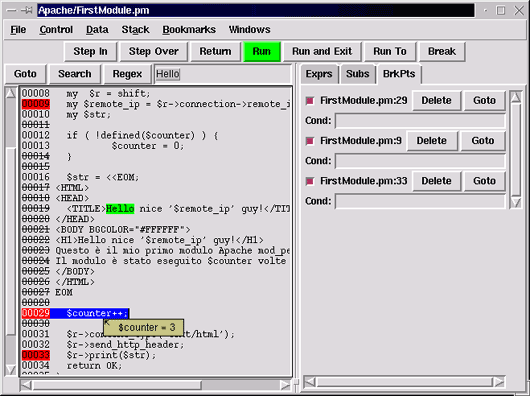
\includegraphics[height=5cm]{ptkdb}
  \end{center}
\end{frame}


\subsection{Object Oriented Perl}

\begin{frame}[containsverbatim]{Vanilla Class Example}
\begin{lstlisting}[caption=A simple class]
package Person;
use strict;
use warnings;

our $VERSION = 0.01;

sub new {
    my ($class, @args) = @_;
    bless { AGE => 0 }, $class;
}

sub age {
    my $self = shift;

    (defined $_[0]) ? $self->{"AGE"} = $_[0] : $self->{"AGE"};
}

1;
\end{lstlisting}
\end{frame}


\begin{frame}[containsverbatim]{Vanilla Class Example (cont.)}
\begin{lstlisting}[caption=Use class]
#!/usr/bin/perl
use strict;
use warnings;
use Person;

my $p = Person->new();
$p->age(20);
print $p->age, "\n";
\end{lstlisting}
\end{frame}


\begin{frame}{RAII - Resource Acquisition Is Initialization}
  \begin{itemize}
    \item   DESTROY() method
    \item   Guard, Scope::Guard, B::Hooks::EndOfScope,
            Hook::Scope, Sub::ScopeFinalizer
  \end{itemize}
\end{frame}

\begin{frame}{Advanced OO}
  \begin{itemize}
    \item   UNIVERSAL
    \item   Class::Struct
    \item   Class::MOP, Moose, Mouse, Any::Moose
  \end{itemize}
\end{frame}

\subsection{Idioms \& Traps}

\begin{frame}{Lazy Perl Programmers}
    \begin{itemize}
        \item   Default argument \$\_
        \item   Omission of parentheses
        \item   Omission of ``->'' in reference of reference: \texttt{\$->[0]\{"name"\}}
        \item   Don't forget readability!
    \end{itemize}
\end{frame}

\begin{frame}[containsverbatim]{Imperious Diamond Operator}
\begin{lstlisting}[caption=Imperious Diamond Operator]
# right
while (<$fh>) {
    # do something with $_
}

# wrong, see perldoc perlvar, /^\s*\$_
while ($not_found && <$fh>) {
    # do something with $_
}
\end{lstlisting}
\end{frame}

\begin{frame}[containsverbatim]{Volatile Capture Buffers}
\begin{lstlisting}[caption=Volatile Capture Buffers]
# wrong
if ( /(\d+)\./ ) {
    print $1 if $1 =~ /^0/;
}

# right
if ( /(\d+)\./ ) {    # or: my ($s) = /(\d+)\./
    my $s = $1;
    print $s if $s =~ /^0/;
}
\end{lstlisting}
\end{frame}


\begin{frame}[containsverbatim]{In-place chomp Function}
\begin{lstlisting}[caption=In-place chomp Function]
# wrong
$s = chomp $s;

# right
chomp $s;
\end{lstlisting}
\end{frame}


\begin{frame}[containsverbatim]{Sticky Iterator}
\begin{lstlisting}[caption=Sticky Iterator]
# wrong
while (my ($k, $v) = each %h) {
    last if $k < 0;
}

while (my ($k, $v) = each %h) {
}

# right
# reset iterator before next iteration with `keys %h' or `values %h'
\end{lstlisting}
\end{frame}


\begin{frame}[containsverbatim]{Innocent Falsehood}
\begin{lstlisting}[caption=Innocent Falsehood]
# wrong
/(\d+)/;
print "Got number!\n" if $1;

# right
/(\d+)/;
print "Got number!\n" if defined $1;
\end{lstlisting}
\end{frame}


\begin{frame}[containsverbatim]{Valuable Exception}
\begin{lstlisting}[caption=Valuable Exception]
# wrong
sub Object::DESTROY {
    eval {}
}

eval {
    my $obj = Object->new();

    die "foo";
}

if ( $@ ) {
    ...
}
# right
...use Try::Tiny...
\end{lstlisting}
\end{frame}

\begin{frame}[containsverbatim]{Unexpected Truth}
\begin{lstlisting}[caption=Unexpected Truth]
# wrong
sub foo {
    ...
    return undef if $error;
}

my @a = foo();      # @a can be (undef) which evaluates to true

# right
sub foo {
    ...
    return if $error;   # returns undef for scalar context,
                        # () for array context, nothing for
                        # void context
}
\end{lstlisting}
\end{frame}


\section{Useful Tricks}
  \subsection{Symbol Table Manipulation}

\begin{frame}[containsverbatim]{HTTP::Server::Simple}
\begin{lstlisting}[caption=HTTP::Server::Simple]
sub run {
    #....
    if ($server) {
        require join( '/', split /::/, $server ) . '.pm';
        *{"$pkg\::ISA"} = [$server];

        # clear the environment before every request
        require HTTP::Server::Simple::CGI;
        *{"$pkg\::post_accept"} = sub {
            HTTP::Server::Simple::CGI::Environment->setup_environment;
            # $self->SUPER::post_accept uses the wrong super package
            $server->can('post_accept')->(@_);
        };
    #....
}
\end{lstlisting}
\end{frame}

  \subsection{Backtracking in Regexes}

\begin{frame}[containsverbatim]{URL Match}
URL = [protocol] host [path [? parameters]]

Task: extract suffix of path or base name if no suffix
\begin{lstlisting}[caption=URL match]
m{
  ^(?:[^:]+.//)?+
  ([^/]++)
  [^?]*
  (?|
     (\.[^?]*)
     |
     /([^?]*)
  )
}x
\end{lstlisting}
\end{frame}

\begin{frame}{URL Match}
  \begin{center}
    Question:

    How to modify the regex to match URLs without path part?
  \end{center}
\end{frame}

\begin{frame}{Recursive Match}
  \begin{center}
    Task: match AB, AABB, AAABBB, ...
  \end{center}
\end{frame}

\begin{frame}[containsverbatim]{Recursive Match}
  \begin{center}
    \lstinline!/^(A(?1)?+B)$/!
  \end{center}
\end{frame}


    \subsection{Happy Programming in Perl}

\begin{frame}{local::lib}
  \begin{itemize}
    \item Try interesting modules without affecting host system
    \item \texttt{cpan>o conf build\_requires\_install\_policy yes}
    \item \texttt{cpan>o conf prerequisites\_policy follow}
    \item \texttt{cpan>o conf commit}
    \item \texttt{cpan>notest install Some::Module}
  \end{itemize}
\end{frame}

\begin{frame}{Other Good Stuffs}
  \begin{itemize}
    \item \url{http://search.cpan.org/dist/Task-Kensho/}
    \item \url{http://search.cpan.org/dist/Inline/}
    \item \url{http://par.perl.org}
    \item \url{http://search.cpan.org/dist/App-perlbrew/}
    \item \url{http://search.cpan.org/dist/Shipwright/}
    \item \url{http://search.cpan.org/dist/Emacs-PDE/}
    \item \url{http://www.vim.org/scripts/script.php?script_id=556}
  \end{itemize}
\end{frame}

\begin{frame}
  \begin{center}
    \_\_END\_\_
  \end{center}
\end{frame}

\end{document}

